% Created 2024-03-15 Fri 09:40
% Intended LaTeX compiler: pdflatex
\documentclass[presentation]{beamer}
\usepackage[utf8]{inputenc}
\usepackage[T1]{fontenc}
\usepackage{graphicx}
\usepackage{longtable}
\usepackage{wrapfig}
\usepackage{rotating}
\usepackage[normalem]{ulem}
\usepackage{amsmath}
\usepackage{amssymb}
\usepackage{capt-of}
\usepackage{hyperref}
\usepackage{minted}
\usepackage{mathpazo}
\usepackage{multicol}
\setbeamertemplate{navigation symbols}{}
\setbeamertemplate{headline}{}
\usetheme{Madrid}
\author{Erik Bäckman}
\date{\today}
\title{DFT och FFT}
\hypersetup{
 pdfauthor={Erik Bäckman},
 pdftitle={DFT och FFT},
 pdfkeywords={},
 pdfsubject={},
 pdfcreator={Emacs 29.2 (Org mode 9.6.15)}, 
 pdflang={English}}
\begin{document}

\maketitle
\section{Intro}
\label{sec:org9548b81}

\begin{center}
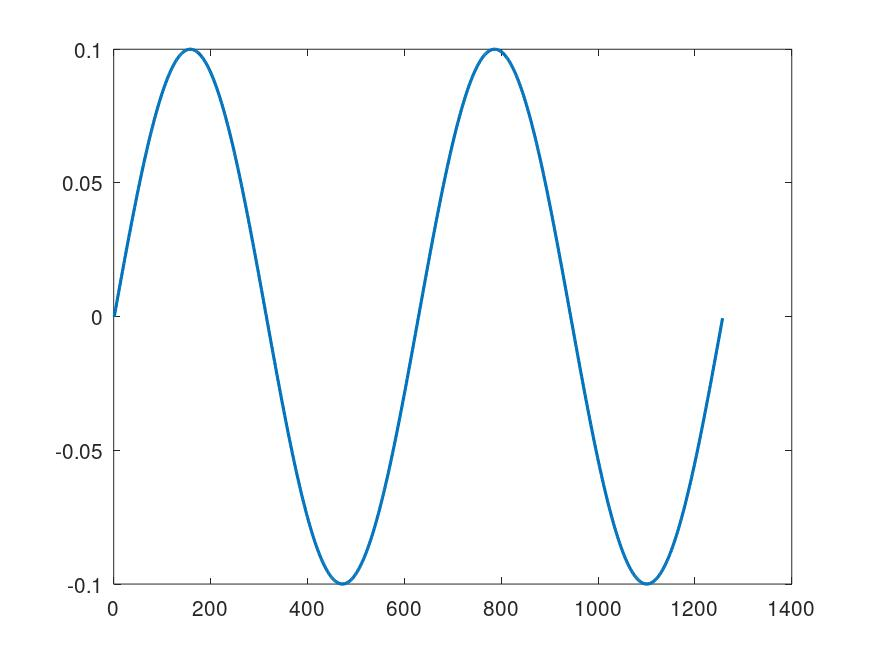
\includegraphics[scale=0.1]{./p1.jpg}
\end{center}  \begin{center}
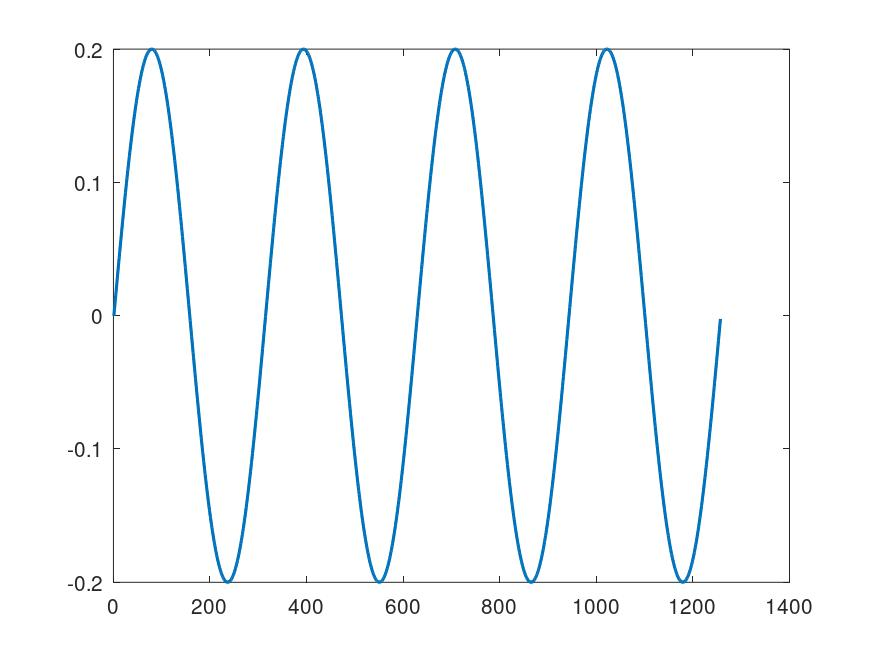
\includegraphics[scale=0.1]{./p2.jpg}
\end{center}
\begin{center}
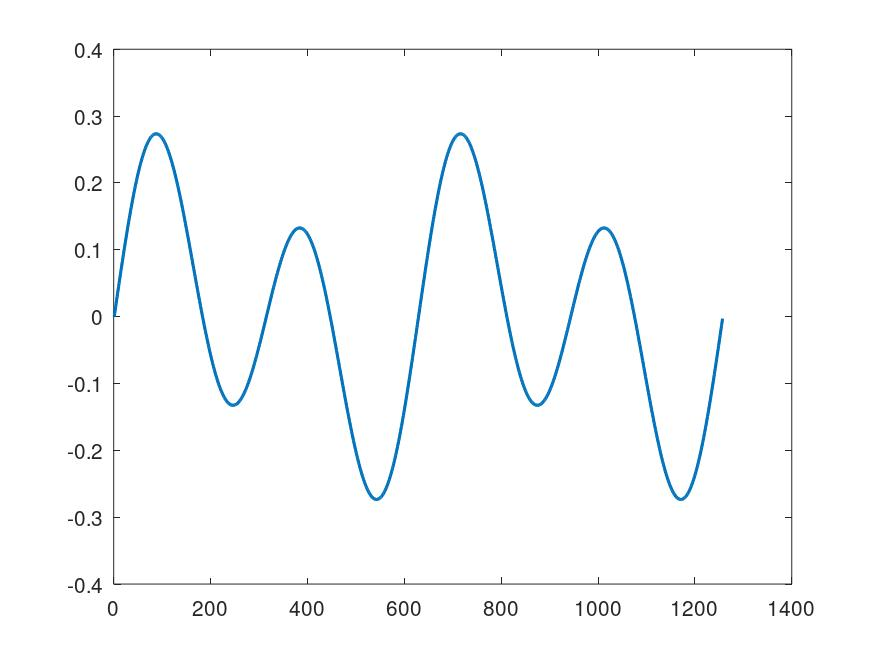
\includegraphics[scale=0.1]{./p3.jpg}
\end{center}

\begin{frame}[label={sec:org3ad615b}]{Fourier Transform}
\[ \hat{f}(u) = \int_{-\infty}^{\infty} f(x)e^{-i2 \pi ut}dt \]
\end{frame}

\begin{frame}[label={sec:org10a2c79}]{DFT}
\begin{equation*}
\begin{aligned}[c]
f &=
  \begin{bmatrix}
    f_{1} \\
    f_{2} \\
    \vdots \\
    f_{N}
    \end{bmatrix}
\end{aligned}
\begin{aligned}[c]
F &=
  \begin{bmatrix}
    \hat{f}_{1} \\
    \hat{f}_{2} \\
    \vdots \\
    \hat{f}_{N}
    \end{bmatrix}
\end{aligned}
\end{equation*}

\begin{align*}
F_{k} &= \sum_{n=0}^{N-1} f_{n} e^{(-i2 \pi nk)/N} \\
      &= A_{k} + B_{k}i
\end{align*}
\end{frame}

\begin{frame}[label={sec:org7fb99f9}]{DFT}
\(N = 4\)

\begin{align*}
  F_{k} &= \sum_{n=0}^{3} f_{n} e^{(-i2 \pi nk)/4} \\
  &= f_{0}w_{4}^{0k} + f_{1}w_{4}^{1k} + f_{2}w_{4}^{2k} + f_{3}w_{4}^{3k}
\end{align*}
\begin{equation*}
w_{N} = e^{-i2 \pi/N}
\end{equation*}
\pause
\begin{gather*}
  \begin{bmatrix}
    \hat{f}_{0} \\
    \hat{f}_{1} \\
    \hat{f}_{2} \\
    \hat{f}_{3}
    \end{bmatrix}
=
\begin{bmatrix}
  w_{4}^{0} & w_{4}^{0} & w_{4}^{0} & w_{4}^{0} \\
  w_{4}^{0} & w_{4}^{1} & w_{4}^{2} & w_{4}^{4} \\
  w_{4}^{0} & w_{4}^{2} & w_{4}^{4} & w_{4}^{6} \\
  w_{4}^{0} & w_{4}^{3} & w_{4}^{6} & w_{4}^{9}
\end{bmatrix}
  \begin{bmatrix}
    f_{0} \\
    f_{1} \\
    f_{2} \\
    f_{3}
    \end{bmatrix}
\end{gather*}
\begin{equation*}
F = Wf
\end{equation*}
\end{frame}

\begin{frame}[label={sec:orga6f6abd}]{DFT}
\begin{equation*}
W =
\begin{bmatrix}
  w_{N}^{0} & w_{N}^{0} & w_{N}^{0} & \dots & w_{N}^{0} \\
  w_{N}^{0} & w_{N}^{1} & w_{N}^{2} & \dots & w_{N}^{N-1} \\
  w_{N}^{0} & w_{N}^{2} & w_{N}^{4} & \dots & w_{N}^{2(N-1)} \\
  \vdots & \vdots & \vdots       & \ddots & \vdots \\  
  w_{N}^{0} & w_{N}^{N-1} & w_{N}^{2(N-1)} & \dots & w_{N}^{(N-1)^{2}}
\end{bmatrix}
\end{equation*}

\begin{equation*}
F = Wf,  \hspace{0.2em} f = W^{-1}F
\end{equation*}

\begin{equation*}
F_{2} = f_{0}e^{-i2 \pi (2)0} + f_{1}e^{-i2 \pi (2)1} + \dots + f_{N-1}e^{-i2 \pi (2)(N-1)}
\end{equation*}
\(N - 1\) komplexa additioner och \(N\) komplexa multiplicationer för \(F_{k}\)
Totalt \(N^{2}\) komplexa multiplicationer. \(O(N^{2})\)
\end{frame}

\begin{frame}[label={sec:org5c34459}]{FFT}
\[ F_{k} = \sum_{n=0}^{N-1} f_{n} \cdot e^{-2 \pi i kn/N}\]
\pause
\[ w_{N} = e^{\frac{-i2 \pi}{N}} \]
\pause
\[ F_{k} = \sum_{n=0}^{N-1} f_{n} \cdot w_{N}^{nk} \]
\end{frame}

\begin{frame}[label={sec:orgd8abace}]{En N-punkt \(F_{k}\) DFT är N-periodisk}
\begin{align*}
&\begin{aligned}
  F_{k} = \sum_{n=0}^{N-1}f_{n} \cdot w_{N}^{nk}
\end{aligned} \\
&\begin{aligned}
  \begin{aligned}
  F_{k+N} &= \sum_{n=0}^{N-1}f_{n} \cdot w_{N}^{n(k+N)} = \sum_{n=0}^{N-1}f_{n} \cdot w_{N}^{nk}w_{N}^{nN} = \sum_{n=0}^{N-1}f_{n} \cdot w_{N}^{nk}e^{(\frac{-i2
          \pi}{N}) nN} \\
        &= \sum_{n=0}^{N-1}f_{n} \cdot w_{N}^{nk}e^{(-i2 \pi)n} =
    \sum_{n=0}^{N-1}f_{n} \cdot w_{N}^{nk} = F_{k}
    \end{aligned}
\end{aligned}
\end{align*}
\end{frame}

\begin{frame}[label={sec:orgf3a2de1}]{Två \(N/2\)-punkt sekvenser med jämna och udda index}
\[
  g_{k} = \left\{f_{0}, f_{2}, f_{4}, \dots, f_{N-2}\right\}, \hspace{0.5em}
  h_{k} = \left\{f_{1}, f_{3}, f_{5}, \dots, f_{N-1}\right\} 
\]

\begin{align*}
F_{k} &= \sum_{n=0}^{N/2 - 1}f_{2n}w_{N}^{2nk} + \sum_{n=0}^{N/2 -
  1}f_{2n + 1}w_{N}^{(2n+1)k} \\
  &= \sum_{n=0}^{N/2 - 1}f_{2n}w_{N}^{2nk} + \sum_{n=0}^{N/2 -
    1}f_{2n+1} w_{N}^{2nk} \cdot w_{N}^{k} \\
    &= \sum_{n=0}^{N/2 - 1}f_{2n}w_{N}^{2nk} + w_{N}^{k} \sum_{n=0}^{N/2 -
      1}f_{2n+1} w_{N}^{2nk} \\
      &= \sum_{n=0}^{N/2 - 1}f_{2n}w_{N/2}^{nk} + w_{N}^{k} \sum_{n=0}^{N/2 -
        1}f_{2n+1} w_{N/2}^{nk} \\
  & = G_{k} + W_{N}^{k}H_{k}
\end{align*}
\end{frame}

\begin{frame}[label={sec:orgf4f9786}]{FFT}
\[ F_{k} = G_{k} + W_{N}^{k}H_{k} \]

\(G_{k}\) och \(H_{k}\) är \(N/2\)-punkt DFTs och därmed \(N/2\) periodiska så
\(G_{k + N/2} = G_{k}\) och \(H_{k + N/2} = H_{k}\).

Dessutom har vi
\[ w_{N}^{k + N/2} = w_{N}^{k}w_{N}^{N/2} = e^{-i2 \pi}w_{N}^{k} = -w_{N}^{k} \]
Så att  

\begin{align*}
&F_{k} = G_{k} + w_{N}^{k}H_{k} \\
&F_{k + N/2} = G_{k} - w_{N}^{k}H_{k}
\end{align*}
\end{frame}

\begin{frame}[label={sec:orge294a38}]{FFT}
Varje steg kräver
\begin{itemize}
\item \(N/2\) komplexa multiplikationer
\item \(N\) komplexa additioner
\end{itemize}

Komplexitet: \(O(N \log_2{N})\)
\end{frame}

\begin{frame}[label={sec:orgba0e8ce},fragile]{FFT: Implementation}
 \begin{minted}[]{julia}
function fft(f)
    N = length(f)
    if N == 1 return f end
    N_half = Int(N/2)
    w = exp(-2π*im/N)
    G = fft(f[1:2:end])
    H = fft(f[2:2:end])
    F = zeros(Complex{Float64}, N)
    wk = 1;
    for k in 1:N_half
        wHk = wk*H[k]
        F[k] = G[k] + wHk
        F[k + N_half] = G[k] - wHk
        wk = wk*w
    end
    return F
end
\end{minted}
\end{frame}

\begin{frame}[label={sec:org7904db4}]{Invers DFT}
\begin{align*}
f_{k} = F_{k}^{-1} = \frac{1}{N}\sum_{n=0}^{N-1}F_{k}e^{\frac{i2 \pi}{N}nk}
\end{align*}
\pause
\begin{equation*}
  F(\bar{F})_{k} = \sum_{n=0}^{N-1}\bar{F_{k}}e^{\frac{-i2 \pi}{N}nk}
\end{equation*}
\pause
\begin{equation*}
  (\overline{F(\bar{F})})_{k} = \sum_{n=0}^{N-1}F_{k}e^{\frac{i2 \pi}{N}nk}
\end{equation*}
\pause
\begin{equation*}
    \frac{1}{N}(\overline{F(\bar{F})})_{k} =
  \frac{1}{N}\sum_{n=0}^{N-1}F_{k}e^{\frac{i2 \pi}{N}nk} = f_{k}
\end{equation*}

\newpage
\end{frame}

\begin{frame}[label={sec:org336728e},fragile]{Invers DFT: Implementation}
 \begin{minted}[]{julia}
function ifft(a)
    a = conj.(a)
    a = fft(a)
    a = conj.(a)
    a = a./length(a)
end
\end{minted}
\end{frame}
\end{document}
